\documentclass[11pt]{article}
\usepackage[english]{babel}
\usepackage{natbib}
\usepackage{url}
\usepackage[utf8x]{inputenc}
\usepackage{amsmath}
\usepackage{graphicx}
\graphicspath{{images/}}
\usepackage{parskip}
\usepackage{fancyhdr}
\usepackage{vmargin}
\usepackage{hyperref}
\usepackage{amsmath}

\title{Asymptotic Equipartition Property}
\author{Gantavya Bhatt}

\begin{document}

\maketitle

\vspace{0.5in}



\section{Problem Statement}

\begin{itemize}
    \item Generate a large number of samples independently from a Bernoulli 
distribution and store the sequence.
\item  Repeat the above procedure, and collect the sequences. Obtain the
Histogram of the distribution of the sequences after collecting a large
number of sequences.
\item As you vary the value of p, observe any structure in the family of
sequences you have generated.
\item Choose a value of \(\epsilon\) to define your own typical set. As you
increase the value of n, observe the fraction of the sequences that lie
in the typical set.
\end{itemize}

\section{Introduction}
This is one of the most important property in the Information theory. Before jumping to the results, we would like to state some expressions that led to the results. 
\subsection{Entropy}
\[ H =  -\sum_{x\epsilon \chi}^{} p(x)log(p(x))\]
\\
For a Bernoulli distribution, this expression reduces to :- \\
\[ H = - (plogp + (1-p)log(1-p))\]

\pagebreak

\begin{center}
        \begin{figure}[!h]
        \centering
          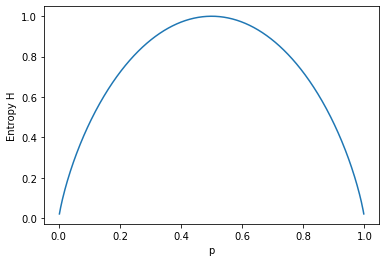
\includegraphics[width=110mm, height=85mm]{Entropy_vs_p.png}
          \caption{ Entropy vs p value
          }
          \label{fig:Piston}
        \end{figure}
\end{center}

\subsection{Weak Law of Large Number}
In probability, the sample mean converges to the true first order moment of the random variable. This can be seen from the limit perspective. 

\[ lim_{N\to\infty} \frac{\sum_{i=1}^{N}X_i}{N} = \mathbcal{E}(X)\]
\\
Experimentally simulating this but for the different expression where X is replaced by log(p(X)) we get the following results. 

\begin{center}
        \begin{figure}[h]
        \centering
          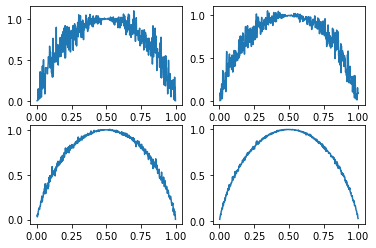
\includegraphics[width=90mm, height=45mm]{WLLN.png}
          \caption{ As N increases, the sample mean converges to Entropy
          }
          \label{fig:Piston}
        \end{figure}
\end{center}
\pagebreak
\section{Typical Set Construction}
We had 3 parameters namely p - the parameter of our bernoulli distribution, N- the length of the Sequence and \(\epsilon\), the convergence threshold. Based on the variation of these parameters, we tabulated our observations and made conclusions out of it. 

\begin{center}
        \begin{figure}[h]
        \centering
          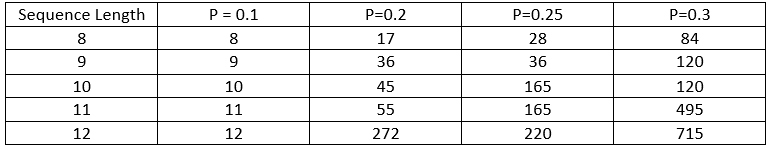
\includegraphics[width=150mm, height=65mm]{Capture.PNG}
          \caption{ The size of the typical set increases with N, and so is with the variation along P. 
          }
          \label{fig:Piston}
        \end{figure}
\end{center}

It can be seen that, as the length of the sequence increases, so is the number of \textbf{unique} elements in the typical set. \\
It can also be seen that as P increases, the entropy increases, hence the size of the typical set increases . 


\begin{center}
        \begin{figure}[h]
        \centering
          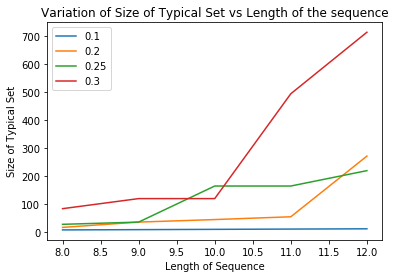
\includegraphics[width=300, height=65mm]{a.png}
          \caption{ Variation of Size of Typical Set
          }
          \label{fig:Piston}
        \end{figure}
\end{center}


\section{Frequency Distribution of Typical Set}

In this section, we are going to make the histogram plot to have a look at the frequency distribution of the Elements in the typical set. For this we are going to plot the decimal values of the Sequence vectors and hence will make their Histogram Plots. 


\begin{center}
        \begin{figure}[!h]
        \centering
          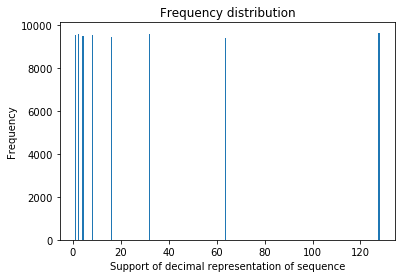
\includegraphics[width=200, height=45mm]{1.png}
          \caption{N=8, \textbf{\(\epsilon=0.15\),} P=0.1}
          \label{fig:Piston}
        \end{figure}
\end{center}

\begin{center}
        \begin{figure}[!h]
        \centering
          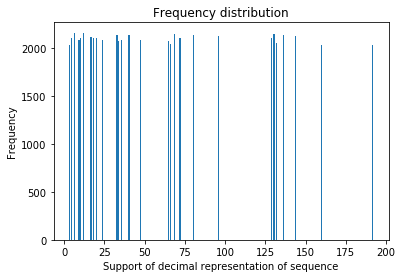
\includegraphics[width=200, height=45mm]{2.png}
          \caption{N=8, \textbf{\(\epsilon=0.15\),} P=0.2}
          \label{fig:Piston}
        \end{figure}
\end{center}

\begin{center}
        \begin{figure}[!h]
        \centering
          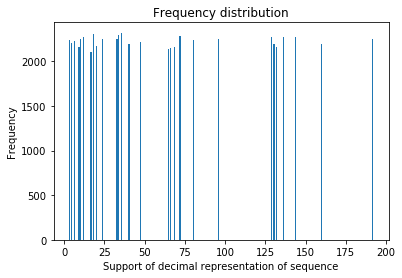
\includegraphics[width=200, height=45mm]{4.png}
          \caption{N=8, \textbf{\(\epsilon=0.15\),} P=0.25}
          \label{fig:Piston}
        \end{figure}
\end{center}

\begin{center}
        \begin{figure}[!h]
        \centering
          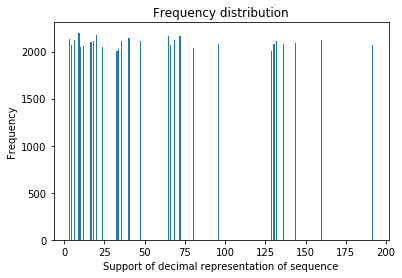
\includegraphics[width=200, height=45mm]{3.png}
          \caption{N=8, \textbf{\(\epsilon=0.08\),} P=0.3}
          \label{fig:Piston}
        \end{figure}
\end{center}

\begin{center}
        \begin{figure}[!h]
        \centering
          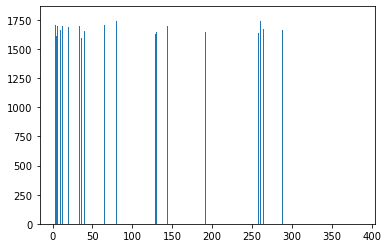
\includegraphics[width=200, height=45mm]{5.png}
          \caption{N=9, \textbf{\(\epsilon=0.05\),} P=0.2}
          \label{fig:Piston}
        \end{figure}
\end{center}

\begin{center}
        \begin{figure}[!h]
        \centering
          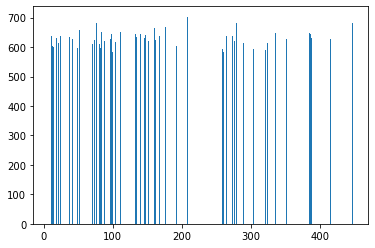
\includegraphics[width=200, height=45mm]{6.png}
          \caption{N=9, \textbf{\(\epsilon=0.05\),} P=0.3}
          \label{fig:Piston}
        \end{figure}
\end{center}

% \begin{center}
%         \begin{figure}[!h]
%         \centering
%           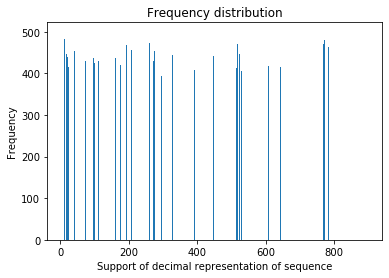
\includegraphics[width=200, height=45mm]{7.png}
%           \caption{N=10, \textbf{\(\epsilon=0.08\),} P=0.3}
%           \label{fig:Piston}
%         \end{figure}
% \end{center}

\pagebreak

\section{Conclusions}
\begin{itemize}
    \item 
Thus from the frequency distribution graph, it was clear that the sequences falling inside the typical set make a more or less uniform distribution.
\item As we increased the length of the sequence, the size of the typical set increased.
\item As we increased the P value, the size of typical set increased.
\item As we decrased the value of \( \epsilon \), the size of the typical set decreased. 
\end{itemize}

Thus, it satisfies the most of postulates of the AEP. 

\section{Further Remarks and Acknowledgement}
The source code can be extended to the source coding schemes and their study. I thank \textbf{Prof Jagdheesh Harshan} for the valuable topics that are covered by him in ELL714- Basic Information Theory. Code available as .ipynb file at following github \textbf{clickable}  
\href{https://github.com/bhattg/Asymptotic_Equipartition_Property}{hyperlink}. 

\end{document}